\documentclass[12pt]{article}
\parindent=0.25in

\setlength{\oddsidemargin}{0pt}
\setlength{\textwidth}{440pt}
\setlength{\topmargin}{0in}
\usepackage{amssymb}
\usepackage{amsfonts}
\usepackage{amsmath}
\usepackage{cancel}
\usepackage{latexsym}
\usepackage[center]{subfigure}
\usepackage{epsfig}
\usepackage{3952}
\usepackage{3952-thm}
\usepackage{pstricks,pst-node,pst-tree}
\usepackage{soul, xcolor}
\usepackage[backref, colorlinks,citecolor=blue,bookmarks=true]{hyperref}  


% \def\size{\mathop{\rm{size}}\nolimits}
% \def\depth{\mathop{\rm{depth}}\nolimits}
% \newtheorem{theorem}{Theorem}
% \newtheorem{lemma}{Lemma}
% \newtheorem{corollary}{Corollary}
% \newtheorem{fact}{Fact}
% \newtheorem{definition}{Definition}
% \newtheorem{claim}{Claim}
% \newenvironment{proof}{\noindent \textbf{Proof:}}{$\Box$}
% \newenvironment{proofsketch}{\noindent \textbf{Proof Sketch:}}
% \newcommand{\infint}{\int_{-\infty}^\infty}
% \newcommand{\intunit}{\int_{-1}^1}
% \newcommand{\binclass}{x \in \{0,1\}^n}
% \newcommand{\example}{\textbf{Example:} }
% \newcommand{\observation}{\textbf{Observation:} }
% \newcommand{\note}{\textbf{Note:} }
% \newcommand{\noisy}[1]{N_\epsilon(#1)}
% \newcommand{\noisens}[1]{ns_\epsilon(#1)}
% \newcommand{\eg}{{\it e.g.,\ }}
% \newcommand{\Inf}{{\mathrm{Inf}}}
% \newcommand{\PAR}{{\mathrm{PAR}}}
% \def\poly{\mathop{\rm{poly}}\nolimits}
% \def\eps{{\epsilon}}
% \newcommand{\E}{{\bf E}}
% \def\through{{,\ldots,}}


\pagestyle{headings}    % Go for customized headings

\newcommand{\handout}[5]{
   \noindent
   \begin{center}
   \framebox{
      \vbox{
    \parbox[t]{4in} {\bf #1 } \vspace{3mm}  {\hfill \bf #2 }
       \vspace{2mm}
       \hbox to 6.00in { {\Large \hfill #5  \hfill} }
       \vspace{1mm}
       \hbox to 6.00in { {\it #3 \hfill #4} }
      }
   }
   \end{center}
   \vspace*{1mm}
}

\hypersetup{linkcolor=magenta}

\begin{document}

\handout{MATH 3952 (Undergraduate Seminar): Quantum Information Theory}{Spring 2024}
{Organizer: Patrick Lei; Presenter: Peri Kay}
{Scribe: Mark Chen}{Lecture 1, Talk 2: January 29, 2024}

\thispagestyle{plain}
% \setcounter{section}{-1}
\section*{Chapter 1 (Ctd.): Quantum Interference}
\section{Qubits, gates, and circuits}
\begin{definition}[Qubits]
There are many quantum objects, such as atoms, trapped ions, molecules, nuclear spins. For any one of them, we can pre-selet two basis states to denote as $\Ket{0}$ and $\Ket{1}$ and use them to implement basic quantum interferences. However we do to achieve this, we call such prepared quantum objects \textbf{quantum biits}, i.e. \textbf{qubits}.
\end{definition}

\begin{definition}[Hadamard Gate]
As we have already used before, one fundamental gate in quantum circuits is the Hadamard gate: $$
H = \frac{1}{\sqrt{2}}\begin{bmatrix}
1 & 1\\
1 & -1
\end{bmatrix}
$$
\end{definition}

\begin{definition}[Quantum Circuit]
Quantum circuits are a convenient way to abstract from all the physics to only zoom in on how the qubits are acted on. The following is such an abstraction of what happens to $\Ket{0}$ qubut as an input in the previous resonant-dispersive-resonant interactions we have seen:
\begin{center}
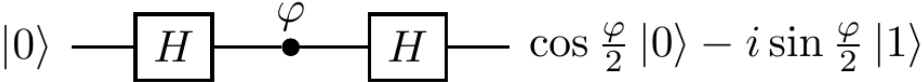
\includegraphics[width = 25em]{images/4.jpg}
\end{center}
We can see that the outcome of the circuit is a superposition of the two possible outcomes, corresponding to what we had seen about the probability amplitudes of $U_{00}$ and $U_{11}$.
\begin{itemize}
    \item (Quantum wires) The lines describe translation in space and time from left to right.
    \item (Quantum (logic) gates) Boxes and circles on the wire, which represent elementary quantum operations; $\eg$ in the circuit diagram above, we have the \underline{Hadamard gates, $H$}, and \underline{phase gate $P_{\varphi} = \begin{bmatrix}
        1 & 0 \\
        0 & e^{i\varphi}
    \end{bmatrix}$}.
\end{itemize}
\end{definition}

\begin{proposition}[Circuits as linear maps]
The circuit diagram is equivalent to the following: $$
HP_\varphi H = \frac{1}{2}\begin{bmatrix}
    1 & 1\\
    1 & -1
\end{bmatrix}\begin{bmatrix}
    1 & 0 \\
    0 & e^{i\varphi}
\end{bmatrix}\begin{bmatrix}
    1 & 1\\
    1 & -1
\end{bmatrix} = \begin{bmatrix}
    \cos\frac{\varphi}{2} & -i \sin\frac{\varphi}{2}\\
    -i \sin\frac{\varphi}{2} & \cos\frac{\varphi}{2}
\end{bmatrix}
$$, where $\varphi = \frac{\varphi_1 - \varphi_0}{2}$ instead of $\frac{\varphi_0 - \varphi_1}{2}$, thus the negative sign on the $\sin$ terms (so, in fact, it is the same as the result from before).

The way $HP_\varphi H$ acts on inputs can be characterized as: $$
\begin{aligned}
\begin{bmatrix}
\Ket{0}\\
\Ket{1}
\end{bmatrix} HP_\varphi H
    &= \begin{bmatrix}
        \Ket{0}\\
        \Ket{1}
        \end{bmatrix}\begin{bmatrix}
            \cos\frac{\varphi}{2} & -i \sin\frac{\varphi}{2}\\
            -i \sin\frac{\varphi}{2} & \cos\frac{\varphi}{2}
        \end{bmatrix} \\
    &\implies \begin{cases}
        \Ket{0}\mapsto \cos\frac{\varphi}{2}\Ket{0} - i\sin\frac{\varphi}{2}\Ket{1}\\
        \Ket{1}\mapsto -i\sin\frac{\varphi}{2}\Ket{0} + \cos\frac{\varphi}{2}\Ket{1}
        \end{cases}
\end{aligned}
$$
\end{proposition}

\section{Quantum Decoherence}
\begin{definition}[Quantum Decoherence]\label{defn:q-d}
Quantum theoretical probability is only useful in a system that is completely isolated; whenever a quantum system interacts with the environment, the superposition collapses into some specific event, in which case the classical probability works just fine. For instance,
\begin{center}
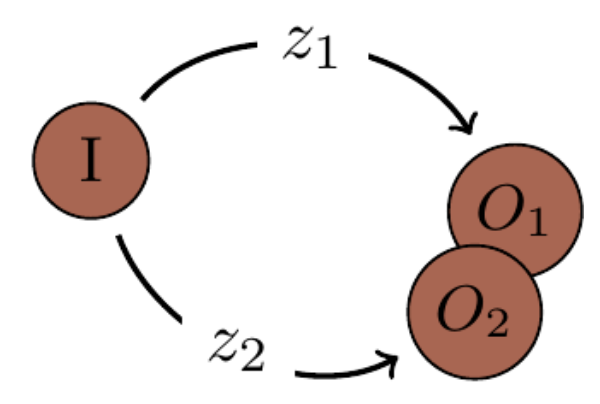
\includegraphics[width = 15em]{images/5.jpg}
\end{center}
would happen if the environment keeps a full physical copy of how the QC reached the output $O$, then the probabilities for these two alternative outcomes would respect classical probability. (If the physical copy of how QC reached $O$ isn't the entire history, it is still possible for the QC to require probability amplitude analysis. But, in either case, we must include the quantum system's interaction with the environment into the probability analysis). Particularly, the example above says:
\begin{itemize}
    \item $O_1$: $O$ was observed and from the environment we know that path $z_1$ was taken.
    \item $O_2$: $O$ was observed and from the environment we know that path $z_2$ was taken.
\end{itemize}
The only difference is which path was taken, which is a question that can be answered without interference. So, the total probability is just $|z_1|^2 + |z_2|^2$.
\end{definition}

\begin{definition}[Visibility Parameter $\&$ Corresponding Terms]
As mentioned in definition \ref{defn:q-d}, the environment may not make the system fully deterministic. So, we introduce the \textbf{visibility} parameter, $v$, and rewrite the original calculation of probability as:$$
P = P_1 + P_2 + 2\boxed{v}\sqrt{P_1P_2}\cos\prt{\varphi_1 - \varphi_2}
$$, where $v\in [0,1]$. Clearly, $v = 0$ means that it is a \textbf{total decoherence}; $v=1$ means that there is \textbf{no decoherence} at all (alternatively, it is a \textbf{full interference}). Any $v\in (0,1)$ would mean that the system is is in a \textbf{partial decoherence}.
\end{definition}

\begin{proposition}
$v$ quantifies the degree of distinguishability between $O_1$ and $O_2$.
\end{proposition}

\begin{proposition}
The more the environment knows about which path was taken, the less interference we see, and the less we can leverage the computational power of quantum effects.
\end{proposition}
\textbf{Intuition:} This should be easy to understand, since when the environment knows all about the interference, the QC is just the same as a normal computer.

\textbf{Why it is useful?} It seems all doomed that when we do decoherence, all the extra powers of QCs are lost. There are several ways to leverage quantum powers while using decoherence, which will be introduced with later concepts, such as \underline{error correction} and \underline{fault-tolerant methods}.

\section{Types of Computation}
\begin{definition}[$n$-qubit input]
Instead of just one single qubit $\Ket{0}$ and $\Ket{1}$, we write $$
\Ket{b_1b_2\cdots b_n}\text{, where }b_1, \ldots, b_n\in \{0,1\}
$$. Analogous to a normal bit-string, this gives a space of all possible such strings of size $2^n$.
\end{definition}

\begin{intuition}\label{int:prob-comp}
Deterministic and probabilistic computation takes the usual definition, but in the context of quantum computation, we have a more analogous way of visualizing what a probabilistic program does:
\begin{center}
    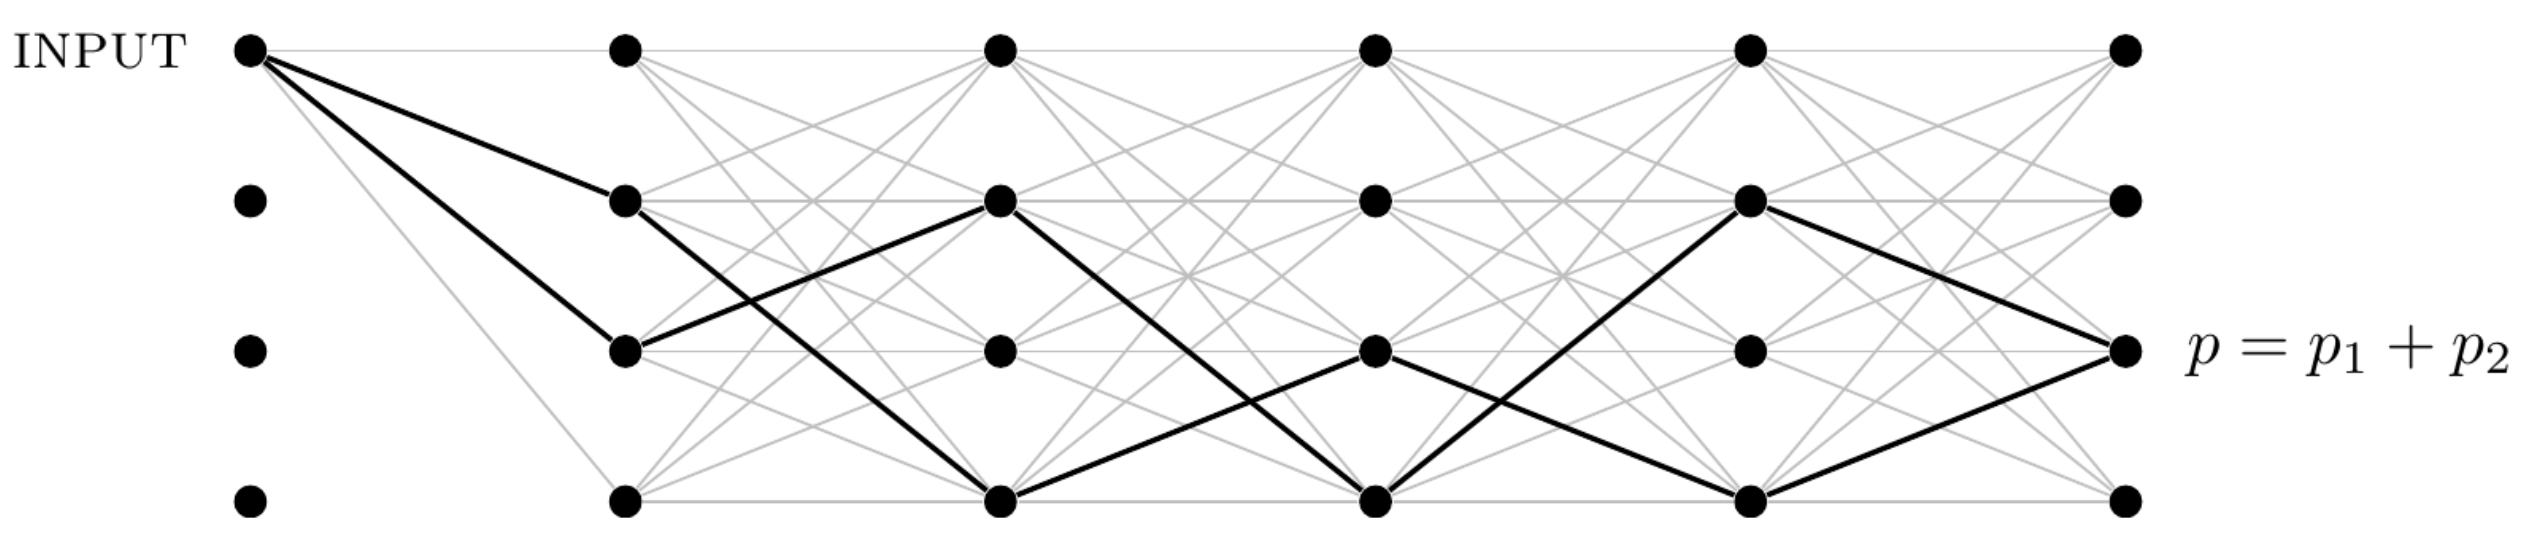
\includegraphics[width = 40em]{images/6.jpg}
\end{center}

The way to verbally describe this is that we start with a specific input string of the whole input space listed as the first column. In this example, we see that it is a space of two-bit string input, and we start with $00$. Then, each step, we change the input by taking certain actions on it (realize that, in this probabilistic model, the action we take can end in different outcomes with a certain probability at each step). Since there are many possible paths that can be taken, it is possible that the algorithm may end in multiple possible outputs. For any specific instance of the output space, the probability of that output being the output of our probabilistic algorithm is the sum of the probabilities of all mutually distinguishable paths.
\end{intuition}

\begin{definition}[Quantum Computation]
The reason why the way to visualize probabilistic algorithms in intuition \ref{int:prob-comp} is a more handy analogy to introducing quantum computation than the typical definition of probabilistic algorithms is because, with this definition, we only need to modify two things:
\begin{itemize}
    \item Each input is a specific $n$-qubit string.
    \item The probability of each instance of the output space is calculated using the quantum theoretic probability that we just introduced - i.e. we add the probability amplitude.
\end{itemize}

Particularly, in quantum computation, we should think of the algorithm to act on the input quantum qubit-string to reach a series of different states to eventually get to the final output. To get the probability of a specific output:
\begin{enumerate}
    \item the probability amplitude of each edge can be specified by the specific action we take - for example, we already know what that probability amplitude change is if the action is a Hadamard gate (since a path consists of a series of steps, we can just multiply them).
    \item Once we know all the mutually exclusive paths that get to a output, the probability amplitude of that output is just the sum of all such paths: $$
    z = \underset{k}{\sum}z_k\implies |z|^2 = \prt{\underset{k}{\sum}z_k}^* \prt{\underset{k}{\sum}z_k} = \underset{k}{\sum}p_k + \underset{k>j}{\sum}2\sqrt{p_kp_j}\cos\prt{\varphi_k - \varphi_j}
    $$
\end{enumerate}
\end{definition}

\subsection{Colloquial summary of quantum computation}
\begin{quote}
``Quantum computation can be viewed as a complex multi-particle quantum interference involving many computational paths through a computing device. The art of quantum computation is to shape the quantum interference through a sequence of computational steps, enhancing probabilities of the “correct” outputs and suppressing probabilities of the ``wrong" ones."
\end{quote}

\section{Computational Complexity}
What we do know is $$
\polytime \subseteq \BPP \subseteq \BQP
$$, while the other direction of containments are all open problems. It is conjectured that $\polytime=\BPP$ and $\polytime \subsetneq \BQP$. One example that is quite strong as a sign to show $\BQP$'s power is FACTORING:
\begin{itemize}
    \item It takes a classic computational model, be it $\polytime$ or $\BPP$ $2^{\Omega(n)}$-time to find prime factorization of a $n$-digit number.
    \item Shor's Algorithm [Peter Shor'94] requires only $O(n^2)$ to prime factorize a $n$-digit number.
\end{itemize}


\end{document}